\documentclass[a4paper,11pt]{article}

% Package imports
\usepackage{amsmath, amssymb, amsthm}
\usepackage{graphicx}
\usepackage{fancyhdr}
\usepackage{geometry}
\usepackage{titlesec}
\usepackage{bm}
\usepackage[nolist]{acronym}
\usepackage[most]{tcolorbox}

\usepackage{needspace} % ensures rule+heading stay together

\newcommand{\rsectionpre}{%
  % Only if not at the top of a page
  \ifdim\pagetotal>0pt
    % If there isn't room for the rule + heading, break first
    \Needspace*{3\baselineskip}%
    % If we didn't break, draw the rule
    \ifdim\pagetotal>0pt
      \noindent\rule{\linewidth}{0.4pt}\par
      \vspace{2em}%
      \nobreak % avoid a break between rule and heading
    \fi
  \fi
}

\newcommand{\rsection}{\section}

% Tell titlesec how to format \ruledsection
\titleformat{\rsection}[block]
  {\rsectionpre\normalfont\Large\bfseries} % format (rule first)
  {\thesection}{1em}{}

% Optional: starred version \ruledsection* (unnumbered)
\titleformat*{\rsection}{\rsectionpre\normalfont\Large\bfseries}

% Page layout
\geometry{left=2cm, right=2cm, top=2.5cm, bottom=2.5cm}
\graphicspath{ {./images/} }

% Header definition
\pagestyle{fancy}
\fancyhf{}
\lhead{Foundations of AI Summary - SS25}
\rhead{\thepage}

% Theorem and definition styles with rounded borders and numbering
\newtcolorbox{definitionbox}{colback=white, colframe=black, arc=5pt, boxrule=1pt, left=5pt, right=5pt, top=5pt, bottom=5pt}
\newtcolorbox{theorembox}{colback=white, colframe=blue, arc=5pt, boxrule=1pt, left=5pt, right=5pt, top=5pt, bottom=5pt}

% Custom commands for numbered definitions and theorems
\newcounter{definitioncounter}
\newcounter{theoremcounter}

\setlength{\parindent}{0pt}
\setlength{\skip\footins}{0.5cm} % Adjust this to change the space above the footnotes
\raggedbottom

\newcommand{\definition}[1]{%
    \refstepcounter{definitioncounter}%
    \begin{definitionbox}
    \textbf{Definition \thedefinitioncounter:}
    \vspace{0.2cm}\newline
    #1
    \end{definitionbox}
    \vspace{0.3cm}
}

\newcommand{\theorem}[1]{%
    \refstepcounter{theoremcounter}%
    \begin{theorembox}
    \textbf{Theorem \thetheoremcounter:}
    \vspace{0.2cm}\newline
    #1
    \end{theorembox}
    \vspace{0.3cm}
}

\newcommand{\cf}[1]{\[#1\]}
\newcommand{\f}[1]{${#1}$}
\renewcommand{\b}[1]{\textbf{#1}}
\renewcommand{\it}[1]{\textit{#1}}
\newcommand{\pL}{\f{\mathcal{L}}}
\newcommand{\fL}{\mathcal{L}}

\begin{document}

\begin{acronym}[AAAAAA]
    \acro{mlp}[MLP]{Multi-Layer-Perceptron}
    \acro{cnn}[CNN]{Convolutional Neural Network}
    \acro{rnn}[RNN]{Recurrent Neural Network}
    \acro{vae}[VAE]{Variational Auto-Encoder}
    \acro{gan}[GAN]{Generative Adversarial Network}
    \acro{bn}[BN]{Batch Normalization}
    \acro{ln}[LN]{Layer Normalization}
    \acro{ml}[ML]{Machine Learning}
    \acro{dl}[DL]{Deep Learning}
    \acro{hpo}[HPO]{Hyperparameter Optimization}
    \acro{bptt}[BPTT]{backpropagation through time}
    \acro{mse}[MSE]{Mean Squared Error}
    \acro{kl}[KL]{Kullback-Leibler}
    \acro{mle}[MLE]{Maximum Likelihood Estimation}
    \acro{relu}[ReLU]{Rectified Linear Unit}
    \acro{sgd}[SGD]{Stochastic Gradient Descent}
    \acro{lstm}[LSTM]{Long Short-Term Memory}
\end{acronym}

% Title section
\begin{center}
    {\huge Foundations of AI - SS25 \par}
    \vspace{0.5cm}
    {\large Niklas Rodenbüsch \par}
    \vspace{0.5cm}
    {\large \today \par}
\end{center}
\vspace{0.5cm}


\section{Rational Agents}
\begin{itemize}
     \item \b{Agent}: Perceives environment through sensors and acts upon it through actuators. Consists of an \it{agent program} running on an \it{architecture}.
     \item \b{Ideal rational agent}: does the "right thing" in terms of a \it{performance measure}.
     \item \b{Rationality} is distinct from \b{omniscience}. An omniscient agent knows the actual effects of its actions, whereas a rational agent acts to maximize its \it{expected} performance based on its percepts and knowledge .
\end{itemize}
\definition{For each possible percept sequence, a \b{rational agent} should select an action that is expected to maximize its performance measure, given the evidence provided by the percept sequence and whatever built-in knowledge the agent has.}

\subsection{Classes of Agents}
\begin{itemize}
     \item \b{Table-Driven:} Use a lookup table indexed by the entire percept sequence to select an action.
     \item \b{Simple Reflex:} React based only on the current percept, using a set of condition-action rules.
     \item \b{Model-based Reflex:} Maintain an internal \it{state} about the world and the effects of its own actions.
     \item \b{Goal-based:} Use explicit \it{goals} to decide on actions, considering how a potential action will bring them closer to their goal.
     \item \b{Utility-based:} When there are multiple possible next actions, a \it{utility function} is used to map a state to a real number.
     \item \b{Learning:} Can improve their performance over time by modifying their behavior. They consist of four main components:
    \begin{itemize}
         \item \b{Performance element:} Selects external actions.
         \item \b{Critic:} Provides feedback on how well the agent is doing based on a performance standard.
         \item \b{Learning element:} Makes improvements to the agent's performance capabilities.
         \item \b{Problem generator:} Suggests actions that can lead to new and informative experiences.
    \end{itemize}
\end{itemize}

\subsection{Types of Environments}
The nature of the environment determines the required complexity of the agent. Some environments are more demanding than others.\\[0.5em]
\b{Most challenging}: Partially observable, nondeterministic, strategic, dynamic, continuous and multi-agent.
\section{Solving Problems by Searching}
Problem-solving agents are a type of goal-based agent that formulates a problem in terms of a \it{state-space} and a \it{goal-state}. Given an \it{initial state} the agent's objective is to find a sequence of actions that leads to the desired goal state. This approach typically assumes the environment is fully observable, deterministic, static, discrete, and single-agent.

\subsection{Concepts}
\begin{itemize}
     \item \b{Transition Model:} Description of the outcome of an action (successor function).
     \item \b{Goal Test:} Tests whether the state description matches a goal state.
     \item \b{Path:} A sequence of actions leading from one state to another.
     \item \b{Problem Type:} Depends on the knowledge of the world states and actions.
     \item \b{Costs:} Specification of search costs (search costs, offline costs) and execution costs (path costs, online costs).
     \item \b{Search Cost:} Time and storage requirements to find a solution.
     \item \b{State Space:} The set of all possible states the environment can be in. This is an abstraction of the real world, containing only relevant details.
     \item \b{Actions:} A set of possible actions available to the agent that can change the world state. Availability of actions might be a function of the state.
\end{itemize}

\subsection{Problem Formulation}
The way a problem is formulated can significantly influence the difficulty of finding a solution! A problem is formally defined as a 5-tuple of: \b{state space, initial state, actions, goal test} and \b{path costs}.

\subsection{Problem Types}
The nature of a problem depends on the agent's knowledge of states and actions.
\begin{itemize}
     \item \b{Completely observable state:} Agent has complete world state and action knowledge. Solution is reduced to searching for a path from the initial state to a goal state.
     \item \b{Partially observable state:} Incomplete world state and action knowledge. The agent only knows which group of world states it is in.
     \item \b{Contingency Problem:} Arises when the choice of action depends on information that will only be available at execution time. The solution must include branching based on (possible) future percepts.
     \item \b{Exploration Problem:} State space and the effects of actions are unknown to the agent.
\end{itemize}
\newpage
\subsection{Search Strategies}
Search algorithms are evaluated based on four criteria:
\begin{itemize}
     \item \b{Completeness:} Is the algorithm guaranteed to find a solution if one exists? 
     \item \b{Optimality:} Does the algorithm find the solution with the lowest path cost? 
     \item \b{Time \& Space Complexity}
\end{itemize}
These are often measured in terms of \f{b} (branching factor), \f{d} (depth of the shallowest goal), and \f{m} (maximum path length in the state space).

\subsection{Uninformed (Blind) Search}
Uninformed search strategies use no information about the distance or cost to the goal.
\begin{itemize}
     \item \b{Breadth-First Search (BFS):} Expands nodes in the order they were generated, exploring layer by layer (FIFO queue). It is complete and is optimal if all action costs are identical. Both time and space complexity are \f{O(b^d)}.
     \item \b{Uniform-Cost Search (UCS):} Expands the node with the lowest path cost, \f{g(n)}, using a priority queue. It finds the optimal solution provided action costs are non-negative.
     \item \b{Depth-First Search (DFS):} Always expands the deepest node first (LIFO queue). It is neither complete nor optimal in general. Its primary advantage is its modest space complexity of \f{O(bm)} in tree-based searches, as it only needs to store the current path.
     \item \b{Depth-Limited Search (DLS):} A variation of DFS that imposes a cutoff on the maximum search depth to prevent infinite paths.
     \item \b{Iterative Deepening Search (IDS):} Combines the benefits of BFS and DFS by running DLS with progressively increasing depth limits. It is complete and optimal (like BFS) but with the low space complexity of DFS (\f{O(bd)}). It is often the preferred uninformed search method when the search space is large and the solution depth is unknown.
     \item \b{Bidirectional Search:} Simultaneously searches forward from the initial state and backward from the goal state. This can drastically reduce time complexity to \f{O(b^{d/2})}. However, it requires reversible operators and an easily definable set of goal states.
\end{itemize}
\vspace{0.5cm}
\begin{figure}[h!]
    \centering
    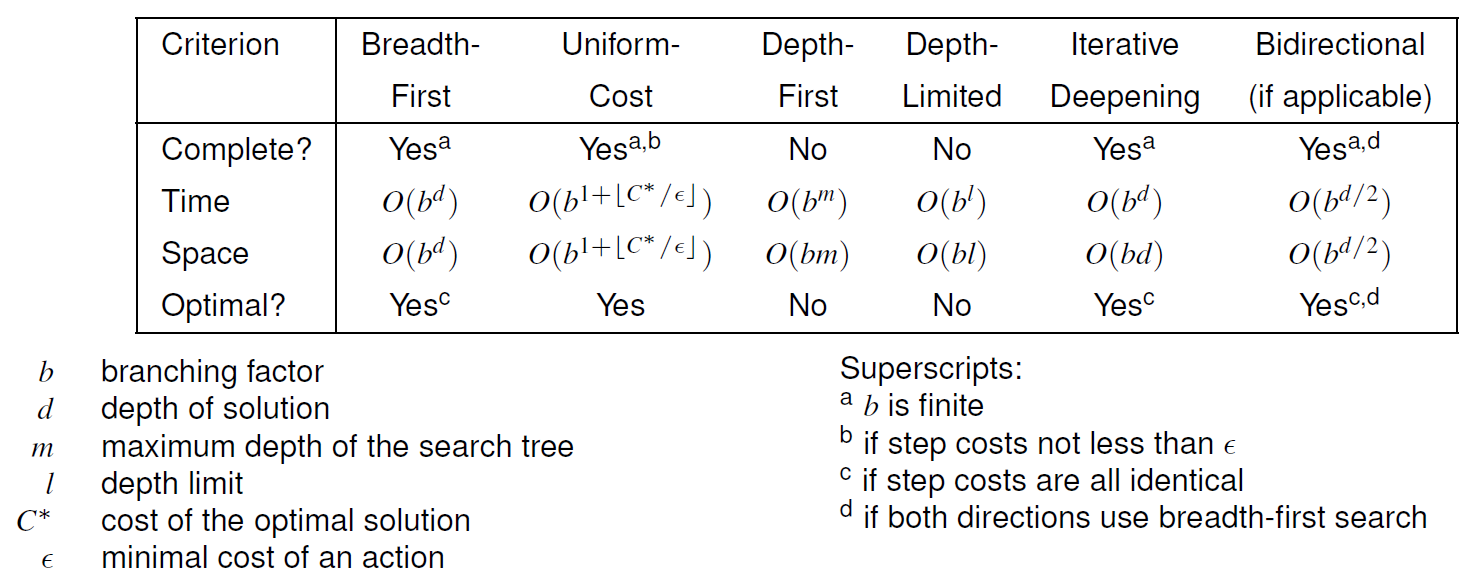
\includegraphics[width=0.7\textwidth]{searches.png}
\end{figure}
\section{Constraint Satisfaction Problems (CSPs)}
 A Constraint Satisfaction Problem (CSP) is a specialized type of search problem where states are defined by assignments of values to a set of variables, and the goal is to satisfy a set of constraints on these variables.

 \definition{A \b{Constraint Satisfaction Problem} is defined by three components :
\begin{itemize}
   \item A set of variables \f{\{x_1, x_2,..., x_n\}}.
   \item A set of domains (values) for each variable \f{\{dom_1, dom_2,..., dom_n\}} \f{\rightarrow d^n} possible assignments 
   \item A set of constraints that specify allowable combinations of values for subsets of variables.
\end{itemize}
 A solution to a CSP is a complete assignment of values to all variables such that all constraints are satisfied. For binary constraints, the problem can be visualized as a \b{constraint graph}, where nodes are variables and edges represent constraints between them.
}

\subsection{Backtracking Search}
 CSPs are often solved using \b{backtracking search}, which is a form of depth-first search. The algorithm incrementally assigns values to variables one at a time, and "backtracks" when a variable has no legal values left to assign.

\subsection{Heuristics \& Pruning Techniques}
Goal: Try to keep the search tree as small as possible and to exploit the CSP problem structure.
\begin{itemize}
  \item \b{Variable Ordering Heuristics:}
  \begin{itemize}
     \item \b{Most-Constrain\it{ed}-Variable:} Choose the variable with the fewest remaining legal values. Helps to detect failures early and directly reduces branching factor.
     \item \b{Most-Constrain\it{ing}-Variable:} As a tie-breaker among variables with the same number of remaining legal values, select the variable that is involved in the most constraints on other unassigned variables. This helps to prune the search tree in future steps.
  \end{itemize}
  \item \b{Value Ordering Heuristics:}
  \begin{itemize}
     \item \b{Least-Constraining-Value:} For a given variable, prefer the value that rules out the fewest choices for the neighboring variables. This leaves more options available, increasing the chance of finding a solution on the current path.
  \end{itemize}
  \item \b{Inference and Constraint Propagation:}
  \begin{itemize}
     \item \b{Forward Checking:} After assigning a value to a variable, check its neighbors and delete any values from their domains that are now inconsistent. If any variable's domain becomes empty, the search can backtrack immediately.
    \item \b{Arc Consistency:} A stronger form of inference. An arc from variable \f{X} to \f{Y} is consistent \it{iff}, for every \f{x\in X}, there is a corresponding value \f{y \in Y} that satisfies the constraint. The \b{AC-3 algorithm} (\f{O(d^3n^2)}) enforces arc consistency throughout the graph. It can be used as a preprocessing step or during search to prune the search space.\\
    \b{Note:} Detecting all inconsistencies is NP-hard!
  \end{itemize}
\end{itemize}

\subsection{Exploiting Problem Structure}
 The structure of the constraint graph can be used to find solutions more efficiently.
\begin{itemize}
   \item \b{Disconnected Components:} If the constraint graph has multiple disconnected components, each can be solved as an independent subproblem.
   \item \b{Tree-Structured CSPs:} If the constraint graph is a tree (i.e., has no loops), the CSP can be solved in polynomial time (\f{O(nd^2)}). This is achieved by ordering the nodes topologically, enforcing arc consistency, and then assigning values from the root down without any need for backtracking.
  \item \b{Almost Tree-Structured CSPs:} For problems that are nearly trees, one can use:
  \begin{itemize}
     \item \b{Cutset Conditioning:} A small set of variables (a "cycle cutset") is chosen to break all loops in the graph. The algorithm tries all consistent assignments for the cutset variables; for each assignment, the remaining problem is a tree and can be solved efficiently.
     \item \b{Tree Decomposition:} The problem is decomposed into a set of connected subproblems, which are organized into a tree. The subproblems are solved, and the solutions are then combined. The efficiency of this method depends on the problem's \it{tree width} \f{w}.
  \end{itemize}
\end{itemize}
\section{Informed Search Methods}
Informed (or heuristic) search strategies use problem-specific knowledge to find solutions more efficiently than uninformed methods. This knowledge is supplied by a \b{heuristic function} \f{h(n)}, which estimates the cost of the cheapest path from a node \f{n} to a goal.

\subsection{Best-First Search}
Best-first search is a general search algorithm that selects the next node to expand based on an \b{evaluation function} \f{f(n)}. It uses a priority queue to always expand the node with the "best" (lowest) \f{f}-value. Different informed search strategies are instances of best-first search with different evaluation functions.

\subsubsection{Greedy Best-First Search}
Greedy search uses only the heuristic function for evaluation: \f{f(n) = h(n)}. It tries to expand the node that it estimates to be closest to the goal. While this approach is often fast, it is not optimal and is generally incomplete.

\subsubsection{A* Search}
A* search combines the benefits of Uniform-Cost Search and Greedy Search. Its evaluation function balances the cost to reach the current node with the estimated cost to get to the goal: 
\cf{f(n) = g(n) + h(n)}
where \f{g(n)} is the known cost of the path from the initial state to node \f{n}, and \f{h(n)} is the heuristic estimate of the cost from \f{n} to the goal.\\
A* is guaranteed to be \b{complete and optimal} if its heuristic function \f{h(n)} is \b{admissible}, meaning it never overestimates the true cost to reach the goal (\f{h(n) \le h^*(n)}). A stronger condition, \b{consistency}, is required for the graph-search version of A* to be optimal without re-opening already visited nodes (consistency implies admissibility). Graph-A* can still be applied if \f{h(n)} is not consistent, but optimality is lost. Drawback: Exponential space complexity, as it must store all generated nodes.\\

\b{Iterative Deepening A* (IDA*)} is a variant that uses the f-cost as a cutoff instead of depth, combining the optimality of A* with the low memory requirements of iterative deepening.

\subsection{Local Search Methods}
For problems where the path to the solution is irrelevant (e.g., 8-queens), local search algorithms can be very effective. These methods operate on a single current state, moving to neighboring states to optimize an objective function. They require very little memory.
\begin{itemize}
    \item \b{Hill-Climbing:} A simple local search that always moves to the best neighboring state. It can get stuck in \b{local maxima}, on \b{plateaus} (flat areas where no neighbor is better), and on \b{ridges}. Can be mitigated by starting over or by injecting noise (random walk).
    \item \b{Simulated Annealing:} An improvement on hill-climbing that can escape local maxima. It allows for "bad" (downhill) moves with a probability (noise) that decreases over time. This probability is controlled by a "temperature" parameter \f{T}, which is gradually lowered according to a schedule.
\end{itemize}

\subsection{Genetic Algorithms}
Genetic Algorithms (GAs) are a class of local search methods inspired by natural evolution. They maintain a \b{population} of candidate solutions (individuals), which are evolved over generations. The core components are:
\begin{itemize}
    \item \b{Fitness Function:} An objective function that evaluates the quality of each individual in the population.
    \item \b{Selection:} Fitter individuals are more likely to be selected to produce offspring.
    \item \b{Crossover:} Creates new individuals by combining genetic material (e.g., parts of bit-strings) from two parents.
    \item \b{Mutation:} Randomly alters parts of an individual, introducing new traits and preventing premature convergence.
\end{itemize}
\section{Board Games}
Board games represent a classic area of AI research, framing the competition between two opponents as a search problem. While the states in a game are fully accessible, they are also contingency problems because a player cannot control the opponent's moves. The primary challenge is the massive size of the game's state space.

\definition{A game can be defined as a 4-tuple of \b{initial state}, \b{operators} (legal moves), a \b{terminal test} and a \b{utility function} (outcome of the game).}

\subsection{Minimax Search}
For two-player, zero-sum games (with players typically called \b{MAX} and \b{MIN}), the \b{minimax algorithm} can determine the optimal move. It assumes that both players play optimally. The algorithm explores the entire game tree to find a move that maximizes the utility for MAX, while assuming MIN will always try to minimize it:\\
The algorithm generates the entire game tree using DFS. A \b{utility function} assigns a value to terminal states of the game (win, loss, or draw). The algorithm propagates these values up the tree: MAX nodes take the maximum value of their children, and MIN nodes take the minimum. MAX then selects the move at the root that leads to the child with the highest value.\\

Since generating the full game tree is often infeasible, the search is typically cut off at a certain depth. The leaf nodes are then scored using an \b{evaluation function} that estimates the desirability of the position. It's best to stop the search only at "quiescent" positions to avoid the \b{horizon effect}, where a critical event is pushed just beyond the search depth limit.

\subsection{Alpha-Beta Pruning}
\b{Alpha-Beta pruning} is an optimization of the minimax algorithm that provides the same result while pruning large parts of the search tree. It eliminates branches that cannot possibly influence the final decision. It maintains two values during the search:
\begin{itemize}
    \item \b{Alpha (\f{\alpha}):} The best (highest) value found so far for MAX on the path to the root.
    \item \b{Beta (\f{\beta}):} The best (lowest) value found so far for MIN on the path to the root.
    \item Prune branches below MIN node where \f{\beta \le \alpha} of its MAX-predecessor. Prune branches below MAX node where \f{\alpha \ge \beta} of its MIN-predecessor.
\end{itemize}
The efficiency of alpha-beta pruning is highly dependent on move ordering. In the best case, it can reduce the effective branching factor from \f{b} to \f{\sqrt{b}}, allowing the search to go twice as deep in the same amount of time.

\subsection{Games with an Element of Chance}
Games like Backgammon involve randomness. To handle this, the standard game tree is augmented with \b{chance nodes}.
\begin{itemize}
    \item These nodes are inserted between the regular MAX and MIN nodes and represent random events, like a dice roll.
    \item Instead of a min or max operation, the value of a chance node is the \b{expected value} of its children, calculated by summing the values of all possible outcomes weighted by their probabilities.
    \item This significantly increases the branching factor and complexity of the search.
\end{itemize}
\newpage
\section{Propositional Logic}
Rational agents often need to represent knowledge about their world to make logical deductions. Propositional logic is a formal language for representing and reasoning with this knowledge.

\subsection{Knowledge-Based Agents}
A knowledge-based agent uses a \b{knowledge base (KB)}, which is a set of sentences expressed in a formal language. The agent can interact with the KB via:
\begin{itemize}
    \item \b{TELL(KB,\f{\alpha})\f{=}KB'} the KB new information it perceives from the environment.
    \item \b{ASK(KB,\f{\alpha})\f{=}yes} the KB what action to take, which is answered by inferring new knowledge from the KB.
\end{itemize}
It is crucial to distinguish between the \b{syntax} of the language (the structure of its sentences) and its \b{semantics} (the meaning or truth of those sentences).

\subsection{Syntax and Semantics of Propositional Logic}
\begin{itemize}
    \item \b{Syntax:} A \b{literal} is an atomic proposition or its negation. A \b{clause} is a disjunction of literals.
    \item \b{Semantics:} The truth of a formula is determined by an \b{interpretation} (or truth assignment), which assigns a truth value (True or False) to each atomic proposition. An interpretation that makes a formula true is called a \b{model} of that formula.
\end{itemize}
A formula can be \b{satisfiable} (has at least one model), \b{unsatisfiable} (has no models), \b{falsifiable} (a model exists that does not satisfy the formula) or \b{valid} (a tautology, true under all interpretations).

\subsection{Logical Entailment and Inference}
\begin{itemize}
    \item \b{Logical Entailment} (\f{\textrm{KB} \models \alpha}): A sentence \f{\alpha} is logically entailed by a knowledge base KB if \f{\alpha} is true in all models of KB. This means that \f{M(\textrm{KB}) \subseteq M(\alpha)}, where \f{M(\phi)} is the set of all models for a formula \f{\phi}.
    \item \b{Inference} (\f{\textrm{KB} \vdash_i \alpha}): Inference is the process of deriving new sentences from existing ones using syntactic rules. A good inference procedure should be:
    \begin{itemize}
        \item \b{Sound:} It only derives sentences that are logically entailed.
        \item \b{Complete:} It can derive all sentences that are logically entailed.
    \end{itemize}
\end{itemize}

\subsection{CNF and DNF}
For every formula, there exists at least one equivalent formula in CNF and one in DNF. A formula in DNF is satisfiable \it{iff} one disjunct is satisfiable.
\cf{
    \textrm{CNF}: \bigwedge^{n}_{i=1}\left(\bigvee^{m_i}_{j=1} l_{i,j} \right) \quad;\quad \textrm{DNF} : \bigvee^{n}_{i=1}\left(\bigwedge^{m_i}_{j=1} l_{i,j} \right)
}
A formula can be turned into CNF by following the steps:
\begin{enumerate}
    \item Eliminate \f{\Rightarrow} and \f{\Leftrightarrow} like so: \f{\alpha \Rightarrow \beta \rightarrow (\neg\alpha \vee \beta)}
    \item Move \f{\neg} inwards: \f{\neg (\alpha \wedge \beta) \rightarrow (\neg\alpha\vee\neg\beta)} (De Morgan's laws)
    \item Distribute \f{\vee} over \f{\wedge} like so: \f{((\alpha\wedge\beta)\vee\gamma)\rightarrow (\alpha\vee\beta)\wedge (\beta\vee\gamma)}
    \item Simplify: \f{\alpha\vee\alpha\rightarrow\alpha} etc.
\end{enumerate}

\subsection{Resolution}
Resolution is a sound and refutation-complete inference rule for deriving new formulae from a KB, that does not depend on testing every interpretation (logical implication).
\begin{itemize}
    \item \b{Goal:} To prove \f{\textrm{KB} \models \alpha}, the resolution algorithm proves that the set of sentences \f{\textrm{KB} \cup \{\neg\alpha\}} is unsatisfiable. This relies on the contradiction theorem.
    \item \b{Requirement:} All sentences must be converted to CNF, which is a conjunction of clauses (disjunctions of literals). Equivalently, we can turn the KB sentences into a set of clauses: 
    \cf{
        \left\{(P\vee Q)\wedge (R\vee \neg P)\wedge S\right\} \rightarrow \left\{\left\{P, Q\right\},\left\{R, \neg P\right\}, \left\{S\right\} \right\}  
    }
    \item \b{The Resolution Rule:} From two clauses containing a complementary literal (e.g., \f{l} and \f{\neg l}), a new clause called the \b{resolvent} is derived. The resolvent contains all literals from the original two clauses except for the complementary pair.
    \cf{\frac{C_1 \cup \{l\}, \quad C_2 \cup \{\neg l\}}{C_1 \cup C_2}}
    \item \b{Proof:} The algorithm repeatedly applies the resolution rule. If the \b{empty clause} (\f{\Box}) is derived, it signifies a contradiction, proving that the original set of clauses was unsatisfiable and thus that \f{KB \models \alpha}.
\end{itemize}
\vspace{0.5em}
\b{Left out:} Special symbols, Interpretation, Implication theorems, Action selection
\section{Satisfiability and Model Construction}
The Boolean Satisfiability Problem (SAT) is a foundational problem in computer science. Given a propositional formula in CNF, the goal is to find a satisfying assignment of truth values (a model) or prove that none exists. Modern SAT solvers provide a highly efficient way to solve many practical NP-hard problems, including hardware/software verification and CSPs.\\
SATs can be formulated as CSPs, where the CSP variables are the symbols of the alphabet, the domain of values is \f{\left\{T,F\right\} }, and the constraints are given by clauses.

\subsection{The DPLL Algorithm}
The \b{Davis-Putnam-Logemann-Loveland (DPLL)} algorithm is a complete and correct backtracking search procedure for solving SAT. It improves upon simple backtracking by using powerful inference rules to prune the search space.
\vspace{0.5em}
\definition{
     Given a set of clauses \f{\Delta} defined over a set of variables \f{\Sigma}, return "satisfiable" if \f{\Delta} is satisfiable, otherwise return "unsatisfiable".
     \begin{enumerate}
          \item If \f{\Delta = \emptyset} return "satisfiable"
          \item If \f{\Box \in \Delta} return "unsatisfiable" (\f{\Box} being the empty clause)
          \item \b{Unit-propagation rule:} If \f{\Delta} contains a unit-clause \f{C}, that is an unassigned literal, assign a truth-value to the variable in \f{C} that satisfies \f{C}, simplify \f{\Delta} to \f{\Delta'} and return DPLL(\f{\Delta'}).
          \item \b{Splitting rule:} When no further progress can be made by unit propagation, select an unassigned variable \f{v} from \f{\Sigma} and recursively try assigning it true and then false. After assigning each truth value, simplify \f{\Delta} to \f{\Delta'} and call DPLL(\f{\Delta'}).
     \end{enumerate}
}

\subsection{Conflict-Driven Clause Learning (CDCL)}
Modern SAT solvers are based on an enhancement of DPLL called \b{Conflict-Driven Clause Learning (CDCL)}.  While DPLL is effective, it "forgets" the reason for a conflict when it backtracks. CDCL improves upon this by learning from its mistakes.  One of its core features is \b{Conflict Analysis and Clause Learning:} When a conflict occurs, the solver analyzes the chain of implications that led to it and generates a new \b{conflict clause}.  This new clause is added to the knowledge base and helps prune the search by preventing the same conflict from recurring.

\definition{
     The CDCL algorithm works as follows:
     \begin{enumerate}
          \item \b{Unit-propagation rule:} If \f{\Delta} contains a unit clause \f{C} for \f{L}, extend the trail with \f{L^C}.
          \item \b{OR:} If there is a conflict, call ANALYZE(conflict):
          \begin{enumerate}
               \item if the learned clause is empty, return "unsatisfiable"
               \item otherwise, backjump: Learn the clause and unit-propagate to the earliest possible split, undoing all splits done later
          \end{enumerate}
          \item \b{Splitting rule:} Select from \f{\Sigma} an unassigned variable \f{v} and assign it a truth value. Extend the trail with \f{L^\dagger }.
          \item If there is no unassigned literal, return "satisfiable(trail)"
          \item Go to step 1
     \end{enumerate}
}
\section{Predicate Logic (PL1)}
While propositional logic is useful, it cannot represent the internal structure of statements or relationships between objects. For example, from "All men are mortal" and "Socrates is a man," it cannot conclude that "Socrates is mortal." First-Order Predicate Logic (PL1) is a more expressive language that overcomes these limitations.

\subsection{Syntax}
PL1 introduces several new syntactic elements:
\begin{itemize}
    \item Quantifiers (\f{\forall}, \f{\exists}), equality (\f{=}), brackets, variables (\f{x, x_1, ..., x', x'', ..., y, z})
    \item \b{Function symbols} (e.g. weight(), color()), lowercase. 0-ary functions are constants.
    \item \b{Predicate symbols} (e.g. Red(), Block()), uppercase. 0-ary predicates are prop. logic atoms.
    \item \b{Terms:} Expressions that represent objects. A term can be a constant, a variable, or a function applied to other terms (e.g., \f{a, x, f(x)}). Terms without variables are called \b{ground terms}.
    \item \b{Atomic formulae:} Represent statements about objects. If \f{t_1, ..., t_n} are terms and \f{P} is an \f{n}-ary predicate, then \f{P(t_1, ..., t_n)} is an atomic formula, so would be \f{t_1=t_2}.
    \item \b{Formulae:} If \f{\phi} and \f{\psi} are formluae and \f{x} ar variable, then every operator application (e.g. \f{\neg\phi}, \f{\phi\wedge\psi}, \f{\exists x\psi}) are formulae. Quantifiers are as strongly binding as \f{\neg}.
\end{itemize}
Formulae with no free variables are called closed formulae or sentences. With closed formulae, variable assignments can be ignored.

\subsection{Semantics:}
The meaning of a PL1 formula is given by an \b{interpretation}, which consists of:
\begin{itemize}
    \item A non-empty \b{domain} \f{D} of objects.
    \item A mapping that assigns objects in \f{D} to constant symbols, functions over \f{D} to function symbols, and relations over \f{D} to predicate symbols.
\end{itemize}
The truth of a formula is evaluated relative to an interpretation and a variable assignment.

\subsection{Reduction to Propositional Logic}
Logical entailment in full PL1 is undecidable, meaning no algorithm exists that can decide for all formulae whether one is entailed by a knowledge base. However, for the special case of a \b{finite domain}, PL1 can be reduced to propositional logic through a process called \b{propositionalization}. This is achieved by first assuming a \b{Domain Closure Axiom}, which states that the only objects in the domain are those named by the constants. Quantifiers are then eliminated through \b{instantiation}:
\begin{itemize}
    \item A universally quantified formula is replaced by a conjunction of the formula with the variable instantiated for every constant in the domain.
    \cf{\forall x \varphi \quad \longrightarrow \quad \varphi[x/c_1] \wedge \varphi[x/c_2] \wedge \dots}
    \item An existentially quantified formula is replaced by a disjunction.
    \cf{\exists x \varphi \quad \longrightarrow \quad \varphi[x/c_1] \vee \varphi[x/c_2] \vee \dots}
\end{itemize}
\b{Notation:} If \f{\varphi} is a formula, then \f{\varphi[x/a]} is the formula with all free occurences of \f{x} replaced by \f{a}.\\[0.5em]
This process results in a (potentially very large) propositional theory that is equivalent to the original PL1 theory and can be solved using standard SAT solvers.
\section{Action Planning}
Planning is the process of finding a sequence of actions to achieve a goal. In AI, this involves declaratively specifying a problem (using logic) — describing the initial state, the available actions, and the goal — and using a domain-independent planner to automatically find a solution.

\subsection{Planning Formalisms}
To describe planning problems in a domain-independent way, formal languages are used.
\subsubsection{STRIPS (STanford Research Institute Problem Solver):}
\begin{itemize}
    \item \b{States} \f{\mathcal{S}} are represented as sets of true propositions (ground atoms), assuming a \b{Closed World Assumption} (any atom not listed is false).
    \item \b{Actions} (or operators) \f{\mathbf{O} } are defined by:
    \begin{itemize}
        \item \b{Preconditions:} A set of propositions that must be true for the action to be executable.
        \item \b{Effects:} A set of propositions that describe how the state changes. This is split into an \b{add list} (atoms that become true) and a \b{delete list} (atoms that become false).
    \end{itemize}
    \item A \b{plan} \f{\Delta} is a sequence of actions that transforms the initial state \f{\mathbf{I} } into a state that satisfies the goal conditions \f{\mathbf{G}}. A \b{planning task} is a 4-tuple \f{\left\langle \mathcal{S}, \mathbf{O}, \mathbf{I}. \mathbf{G}\right\rangle }.
\end{itemize}

\subsubsection{PDDL (Planning Domain Description Language):}
The de facto standard language for planning problems. It extends STRIPS with more expressive features like typing, conditional effects, and numerical resources.

\subsection{Basic Planning Algorithms}
Planning can be framed as a search problem on a state-transition graph. Here, nodes are defined by value assignments to states and labeled edges are the actions that change the appropriate nodes.
\begin{itemize}
    \item \b{Progression Planning (Forward Search):} This approach searches forward from the initial state towards a goal state. At each step, it considers all applicable actions and generates successor states. This is intuitive and easy to implement.
    \item \b{Regression Planning (Backward Search):} This approach searches backward from the goal description towards the initial state. It starts with the goal and determines what conditions must have been true before an action was taken to achieve it. This can be more efficient as it only considers actions relevant to the goal.
\end{itemize}

% \subsection{Complexity and Modern Approaches}
% Action planning is computationally difficult.
% \begin{itemize}
%     \item \b{Complexity:} For propositional STRIPS, finding a plan is \b{PSPACE-complete}. If the plan length is bounded by a polynomial, the problem is \b{NP-complete}. With unrestricted function symbols, planning is \b{undecidable}.
%     \item \b{Planning as Satisfiability:} One powerful modern approach is to translate a planning problem into a Boolean Satisfiability (SAT) problem. The problem is encoded such that any satisfying assignment to the Boolean formula corresponds to a valid plan. This is typically done for a fixed plan length, which is iteratively increased.
%     \item \b{Heuristic Forward Search:} Currently one of the most dominant approaches. It performs a forward search guided by a strong, automatically derived heuristic. A common technique is to use a \b{relaxed problem} to generate the heuristic. For example, the "delete relaxation" ignores all negative effects of actions. The cost of solving this simpler problem provides a powerful (and admissible) heuristic for guiding the search in the original problem.
% \end{itemize}
\section{Making Decisions Under Uncertainty}
Agents in the real world must often act with incomplete or uncertain information. Logical rules can be brittle, as it's impossible to list all preconditions for an action (the qualification problem) or all possible causes for an effect. Probability theory provides a formal framework for representing and reasoning with an agent's degree of belief in the face of uncertainty. When combined with utility theory, it forms the basis of \b{decision theory}, which allows an agent to choose actions that maximize its expected utility.

\subsection{Foundations of Probability Theory}
Probability is governed by a set of axioms, from which all other properties are derived.
\begin{itemize}
    \item An \b{unconditional (or prior) probability} \f{P(A)} represents the degree of belief in a proposition \f{A} in the absence of other information.
    \item A \b{conditional (or posterior) probability} \f{P(A|B)} represents the belief in \f{A} given that evidence \f{B} is known.
    \item The \b{Product Rule} states: \f{P(A \wedge B) = P(A|B)P(B) = P(B|A)P(A)}.
    \item \b{Independence:} \f{a} and \f{b} are independent \it{iff} \f{P(a|b) = P(a)} (\f{\Rightarrow P(a\wedge b) = P(a)P(b)})
    \item \b{Bayes' Rule} is a cornerstone of probabilistic reasoning, allowing us to update beliefs based on new evidence. It relates causal and diagnostic knowledge:
    \cf{P(\text{cause}|\text{effect}) = \frac{P(\text{effect}|\text{cause})P(\text{cause})}{P(\text{effect})}}
\end{itemize}

\subsection{Probabilistic Inference}
The \b{joint probability distribution} specifies a probability for every possible state of the world (i.e., every complete assignment of values to all random variables, like in a probability table). In a probability table the sum of all fields is 1 (disjunction of events). The probability for any random variable can be computed from the joint distribution through \b{marginalization} (summing out variables over rows or columns). Conditional probabilities can be obtained using marginal probabilities.

To make probabilistic inference feasible, we rely on \b{conditional independence}. Two variables \f{A} and \f{B} are conditionally independent given \f{C} if \f{P(A|B,C) = P(A|C)}. This means that once we know the outcome of \f{C}, learning about \f{B} provides no additional information about \f{A}.

\subsection{Bayesian Networks}
A \b{Bayesian Network} is a powerful tool for representing and reasoning with uncertain knowledge. It provides a compact representation of the joint probability distribution by making explicit the conditional independence relationships in a domain.
\begin{itemize}
    \item \b{Structure:} A network is a \b{Directed Acyclic Graph (DAG)} where nodes represent random variables and directed edges represent direct causal influences.
    \item \b{Parameters:} Each node has an associated \b{Conditional Probability Table (CPT)} that quantifies the probability of that node's value given the values of its parent nodes.
    \item \b{Semantics:} A Bayesian network encodes the assumption that each node is conditionally independent of its non-descendants, given its parents. This allows the full joint probability to be factored into a product of local conditional probabilities:
    \cf{P(x_1, \dots, x_n) = \prod_{i=1}^n P(x_i | \text{parents}(x_i))\quad,}
    where \f{X_1, ..., X_n} are the topologically ordered nodes and \f{x_1, ..., x_n} are the values of the variables.
    \item \b{Inference:} The primary task is to compute the posterior probability of a query variable given some observed evidence \f{e}. The network gives a complete representation of the full joint distribution. A query can be answered by computing sums of products of conditional probabilities (summing over the hidden variables). Exact inference is generally NP-hard (approximation via MCMC). Worst-case time complexity is \f{O(2^n)} for \f{n} boolean variables. For singly connected graphs and polytrees, time and space complexity is linear in the number of nodes.
\end{itemize}
\vspace{0.5cm}
\b{Left out:} ENUMERATION-ASK, Bayesian updating
\section{Acting Under Uncertainty}
When an agent operates in a stochastic environment, it must consider the uncertainty of action outcomes. Decision theory, which combines utility theory and probability theory, provides a framework for making rational choices by selecting actions that maximize the agent's expected utility.

\subsection{Utility Theory and the MEU Principle}
\begin{itemize}
    \item A \b{utility function} \f{U(S)} assigns a numerical value to each state \f{S}, representing its desirability to the agent.
    \item The axioms of utility theory (e.g., Orderability, Transitivity, Continuity) provide a foundation for rational preferences. If an agent's preferences conform to these axioms, a utility function that represents those preferences is guaranteed to exist.
    \item The \b{Principle of Maximum Expected Utility (MEU)} states that a rational agent should choose the action that maximizes its expected utility. The expected utility of an action \f{A} given evidence \f{E} is calculated as:
    \cf{EU(A|E) = \sum_{i} P(\text{Result}(A)=i | \text{Do}(A), E) U(i)}
    Problem: The probability part of MEU requires a complete causal model of the world (e.g. requiring constant belief network updating, NP-hard), while the utility part of MEU requires search or planning.
\end{itemize}

\subsection{Sequential Decision Problems and MDPs}
Many problems require an agent to make a sequence of decisions over time. A \b{Markov Decision Process (MDP)} is a formal model for sequential decision-making in a fully observable, stochastic environment. An MDP is defined by:
\begin{itemize}
    \item A set of states \f{S}.
    \item A set of actions \f{A}.
    \item A \b{transition model} \f{P(s'|s,a)}, giving the probability of reaching state \f{s'} from state \f{s} after taking action \f{a}.
    \item A \b{reward function} \f{R(s)}, specifying the immediate reward received in state \f{s}.
\end{itemize}
A \b{policy}, \f{\pi(s)}, is a mapping from states to actions. The goal is to find the \b{optimal policy}, \f{\pi^*}, which maximizes the long-term expected reward. For finite horizon problems, \f{\pi*} depends on current state and remaining steps to go (nonstationary). For inifite horizon problems, it only depends on the current state (stationary).

\subsection{The Bellman Equation and Algorithms for MDPs}
The long-term utility of a state, \f{U(s)}, is the expected sum of future discounted rewards, using a discount factor \f{\gamma \in [0, 1)}. The relationship between the utility of a state and its successors is defined by the \b{Bellman Equation}:
\cf{U(s) = R(s) + \gamma \max_a \sum_{s'} P(s'|s, a) U(s')}
This equation is the foundation for algorithms that solve MDPs. The agent simply chooses the action that maximizes the expected utility of the subsequent state:
\cf{
    \pi(s) = \arg\max_a\sum_{s'}P(s'|s,a)U(s')
}
\begin{itemize}
    \item \b{Value Iteration:} An iterative algorithm that calculates the optimal utility for each state. It starts with arbitrary utilities and repeatedly applies the Bellman update until the values converge. Bellman update:
    \cf{
        U'(s) \leftarrow R(s) + \gamma \max_a \sum_{s'} P(s'|s, a) U(s')
    }
    \item \b{Policy Iteration:} An alternative algorithm that often converges faster. It alternates between two steps until the policy becomes stable: (1) \b{Policy Evaluation}, where given a policy \f{\pi_t} it calculates the utilities for the current policy \f{U_t=U^{\pi_t}}, and (2) \b{Policy Improvement}, where it uses these utilities to create a better policy according to:
    \cf{\pi_{t+1}(s)=\arg\max_a\sum_{s'}P(s'|s,a)U_t(s')}
\end{itemize}
\vspace{0.5cm}
\b{Left out:} Concrete utility theory axioms
\newpage
\section{Machine Learning}
An agent is said to learn if it improves its performance on a task with experience. Machine learning provides the tools for agents to adapt and improve automatically, rather than being explicitly programmed for every possible scenario. A learning agent is typically composed of a performance element (which acts), a learning element (which improves), a critic (which provides feedback), and a problem generator (which suggests exploratory actions).

\subsection{Types of Learning}
Machine learning is often categorized by the type of feedback the agent receives.
\begin{itemize}
    \item \b{Supervised Learning:} The agent learns a function from a training set of labeled input-output pairs \f{\{(x_1, y_1), \dots, (x_N, y_N)\}}. The goal is to find a hypothesis \f{h} that can generalize from this data to accurately predict the output for unseen inputs. \\
    A key principle in supervised learning is \b{Ockham's razor}, which advocates for choosing the simplest hypothesis that is consistent with the data.
    \item \b{Reinforcement Learning:} The agent learns from rewards or punishments (reinforcement signals). It is not told which action to take but must discover a policy that maximizes its cumulative reward over time through trial and error.
    \item \b{Unsupervised Learning:} The agent learns patterns directly from unlabeled data, without any explicit feedback.
\end{itemize}

\subsection{Decision Trees}
A decision tree is a simple yet powerful model used for classification and regression. It represents a function that takes a set of input attributes and returns a decision.
\begin{itemize}
    \item \b{Structure:} The tree consists of internal nodes that test an attribute, branches corresponding to the attribute's values, and leaf nodes that specify the final output or classification.
    \item \b{Learning Algorithm:} Finding the smallest possible decision tree is an intractable problem. Instead, a greedy, divide-and-conquer algorithm is used to build the tree:
    \begin{enumerate}
        \item If all examples in the current subset have the same classification, create a leaf node.
        \item Otherwise, select the "best" attribute to split the examples into smaller subsets.
        \item Recurse on each subset.
    \end{enumerate}
    \item \b{Attribute Selection:} To choose the "best" attribute for a split, the algorithm calculates the information gain for each attribute. Information gain measures the reduction in uncertainty, or \b{entropy}, after the split. The attribute with the highest information gain is chosen. Entropy is defined as:
    \cf{I(P(y_1), \dots, P(y_n)) = \sum_{i=1}^n -P(y_i) \log_2 P(y_i)}
\end{itemize}

\subsection{Assessing Performance}
To evaluate a learning algorithm, it is crucial to separate the data into a \b{training set} and a \b{test set}. The training set is used to learn the hypothesis (e.g., build the decision tree), while the test set, which the model has never seen, is used to evaluate its performance and generalization ability.\\
A \b{learning curve} can be plotted to show how the model's performance on the test set improves as the size of the training set increases.
\section{Deep Learning}
Deep learning is a subfield of machine learning that has achieved state-of-the-art results across a wide range of tasks, including computer vision, speech recognition, natural language processing, and playing complex games like Go.

\subsection{Representation Learning}
Traditional machine learning pipelines often require extensive manual \b{feature engineering} to transform raw data (like images or text) into a suitable representation from which a model can learn.
\begin{itemize}
    \item \b{Representation Learning} refers to a set of methods that automatically discover the necessary features or representations from raw data.
    \item \b{Deep Learning} is a form of representation learning that uses models with multiple layers to learn a \b{hierarchy of features}. Each layer transforms the input from the previous layer into a more abstract and complex representation.
\end{itemize}

\subsection{Multilayer Perceptrons (MLPs)}
\begin{itemize}
    \item \b{Structure:} An MLP consists of an input layer, one or more \b{hidden layers}, and an output layer. Each layer contains interconnected nodes called neurons.
    \item \b{Computation:} The output of each neuron is calculated by taking a weighted sum of its inputs, adding a bias, and then passing the result through a non-linear \b{activation function}. Common activation functions include the logistic sigmoid, tanh and ReLU.
    \item \b{Training:} The network's parameters (weights and biases) are learned by minimizing a loss function that measures the discrepancy between the network's predictions and the true labels. This is typically done using \b{Stochastic Gradient Descent (SGD)}. The gradients required for this optimization are calculated efficiently using the \b{backpropagation} algorithm.
\end{itemize}

\subsection{Advanced Architectures}
\begin{itemize}
    \item \b{Convolutional Neural Networks (CNNs):} CNNs are specialized for processing grid-like data, such as images. They use a mathematical operation called \b{convolution}, where a small filter (or kernel) is slid across the input. This allows the network to efficiently learn a hierarchy of local patterns (e.g., edges, textures, shapes) while sharing parameters, making them highly effective for computer vision tasks.
    \item \b{Recurrent Neural Networks (RNNs):} RNNs are designed to handle sequential data, like text or time series. They have loops in their structure that create an internal state or "memory," allowing them to process sequences of arbitrary length. However, they can be difficult to train on long sequences due to issues like vanishing or exploding gradients.
    \item \b{Transformers:} A more modern architecture that has become dominant in natural language processing. Instead of processing sequences step-by-step like RNNs, Transformers use an \b{attention mechanism} to weigh the importance of all input elements simultaneously. This allows them to capture long-range dependencies in data much more effectively.
\end{itemize}


\end{document}
